% Copyright 2015 http://www.highschoolmathandchess.com/
% This program is free software: you can redistribute it and/or modify
%   it under the terms of the GNU General Public License as published by
%    the Free Software Foundation, either version 3 of the License, or
%    (at your option) any later version.
%    This program is distributed in the hope that it will be useful,
%   but WITHOUT ANY WARRANTY; without even the implied warranty of
%   MERCHANTABILITY or FITNESS FOR A PARTICULAR PURPOSE.  See the
%    GNU General Public License for more details.
%
%    You should have received a copy of the GNU General Public License
%    along with this program.  If not, see <http://www.gnu.org/licenses/>.
%
\documentclass{standalone} 
\usepackage{pgfplots}  
\pgfplotsset{compat = newest}%avoids potential bugs in older versions
\usepgfplotslibrary{dateplot}  
\pgfkeys{
  /pgf/number format/set thousands separator =
}%avoids the year being formatted with a comma; eg, 1,980
\usepackage{xcolor}
\pagestyle{empty}
\begin{document} 
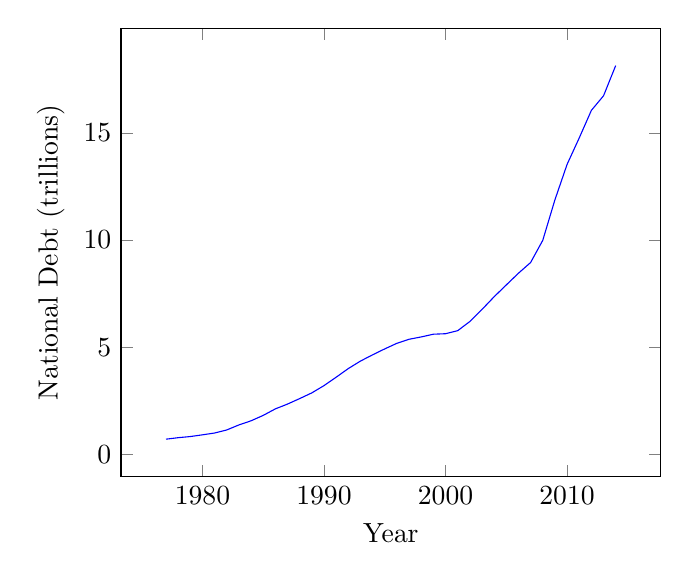
\begin{tikzpicture}
\begin{axis}[
scaled y ticks = false,
xlabel=Year,
ylabel=National Debt (trillions)
]
\addplot[blue, mark size=0.17pt] coordinates {
(1977,.706)
(1978,.776)
(1979,.829)
(1980,.909)
(1981,.994)
(1982,1.137)
(1983,1.371)
(1984,1.564)
(1985,1.817)
(1986,2.120)
(1987,2.345)
(1988,2.601)
(1989,2.867)
(1990,3.206)
(1991,3.598)
(1992,4.001)
(1993,4.351)
(1994,4.643)
(1995,4.920)
(1996,5.181)
(1997,5.369)
(1998,5.478)
(1999,5.605)
(2000,5.628)
(2001,5.769)
(2002,6.198)
(2003,6.760)
(2004,7.354)
(2005,7.905)
(2006,8.451)
(2007,8.951)
(2008,9.986)
(2009,11.876)
(2010,13.529)
(2011,14.764)
(2012,16.051)
(2013,16.732)
(2014,18.141)
};
\end{axis}
\end{tikzpicture}
\end{document}